\documentclass[10pt]{exam}
\usepackage[phy]{template-for-exam}
\usepackage{tikz}
\usepackage[top=0.2in, bottom=0.5in, left=1in, right=1in]{geometry}


\begin{document}
\pagestyle{empty}

\def\mytitle{Unit 04 Test: Forces}

\newcommand{\topmatter} {
  \vspace{2em}
  {\noindent \Large \bf Instructions:}

  \vspace{1em}

  \noindent {\bf Please do not open this test until told to do so!}

  \begin{itemize}
    \item Put your name on this page
    \item Bubble in the number that is on your class notebook where it says ``ZipGrade ID''
    \item When instructed, tear off this first page
    \item Write your answers to the free-response questions on the back of this page.
    \item Bubble in your answers to the multiple-choice questions here.
    
  \end{itemize}

}
\newcommand{\bottommatter}{
  
\begin{tikzpicture}
    \draw (-0.3,0) -- (0.3,0) -- (0,0.530) -- cycle;
    \node at (0,0.2) {\bf !};
  \end{tikzpicture}
  \bf Don't forget to do the problems on the back of this page!
}

\newcommand{\drawscantron}[2]{
  \begin{flushright}
    \begin{tikzpicture}
      \node[anchor=south west] at (0,0) {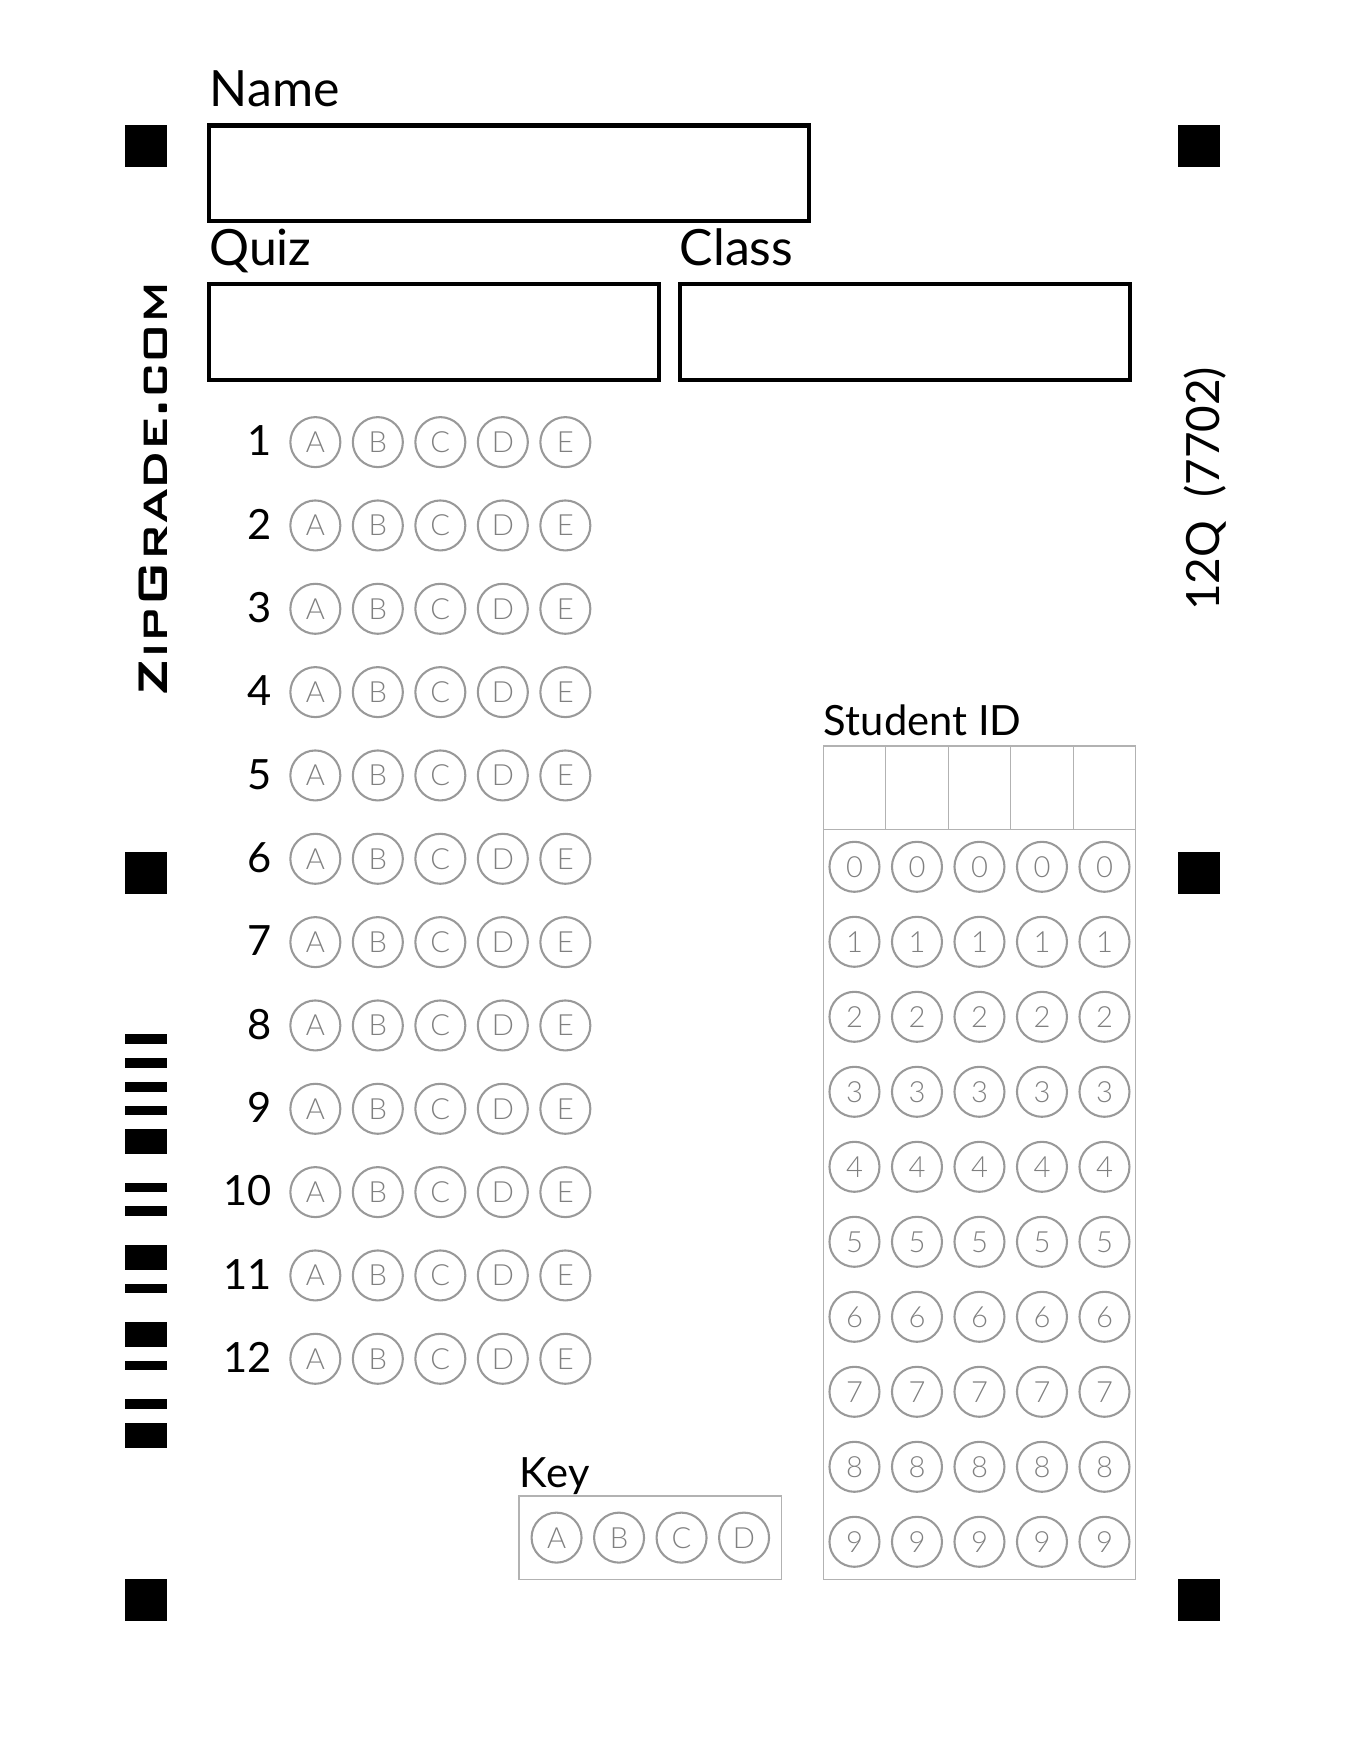
\includegraphics[width=.7\textwidth]{scantron.png}};
      \fill (#1,#2) circle (0.25);
      \node[anchor=west] at (2,12.25) {\small \mytitle};
      \fill[white] (7.2,8.8) rectangle (8.25,1.5);
      \node[fill=white] at (8.4,9.05) {\bf ZipGrade ID:};
    \end{tikzpicture}
  
    \bottommatter
  \end{flushright}
}



  \drawscantron{4.9}{1.9}
  \topmatter

\pagebreak

  \drawscantron{5.45}{1.9}
  \topmatter



\end{document}